\documentclass[a4paper,12pt]{article}
\usepackage{listings,graphicx}
\begin{document}
\title{「プログラミング言語」\\
第3回課題}
\author{工学部情報学科\\
平成25年入学\\
学籍番号:1029-25-2723\\
森井 崇斗 }
\date{\today}
\maketitle

\lstset{numbers=left,basicstyle=\ttfamily\small,
  commentstyle=\textit, keywordstyle=\bfseries}

  \section{問題3.7}
  \subsection{考え方}
  make-jointが返却する手続き内で新たなパスワードの正しさを確認した後に、元の口座のパスワードを利用して元の口座を変更する手続きを呼び出すようにすれば良い。
  \subsection{プログラム}
  \lstinputlisting{3-7.scm}
  \subsection{実行例}
  \lstinputlisting{3-7sample.txt}

  \section{問題3.9}
  \subsection{再帰版の環境構造}
  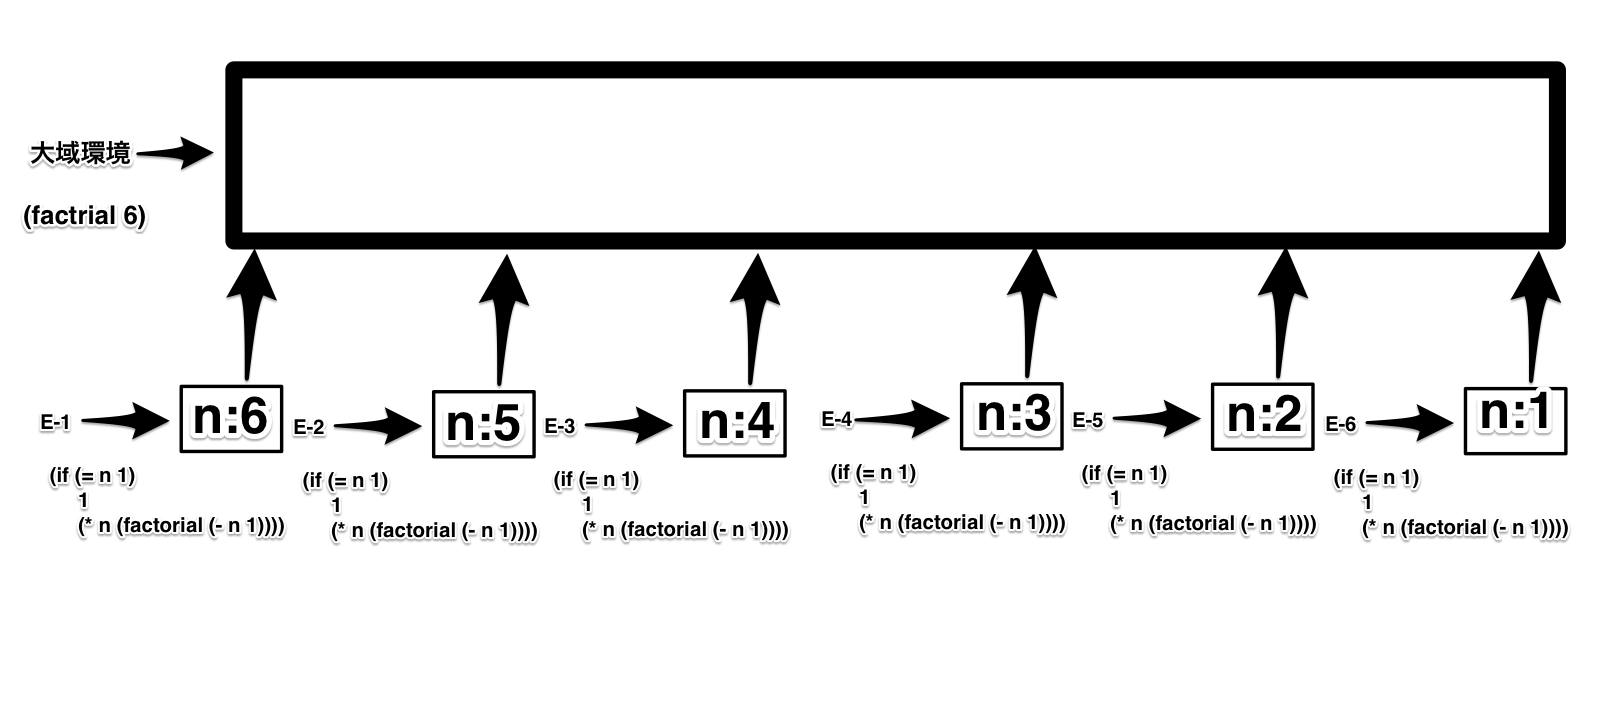
\includegraphics[width=15cm]{factrial.eps}

  \subsection{反復版版の環境構造}
  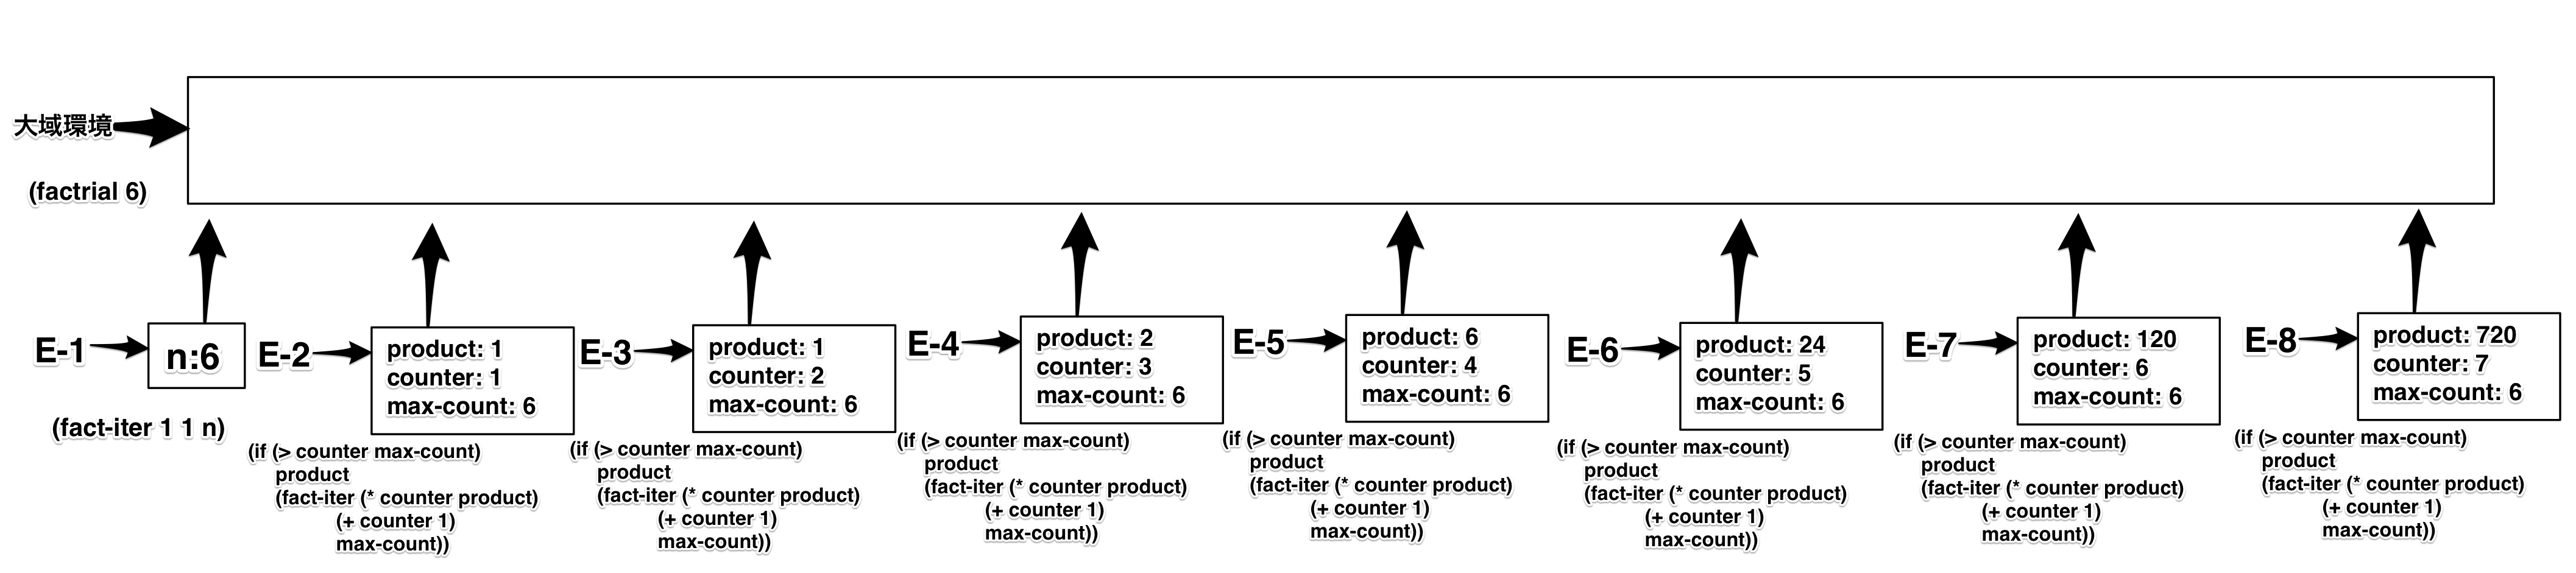
\includegraphics[width=15cm]{iter.eps}

  \section{Check Point}

  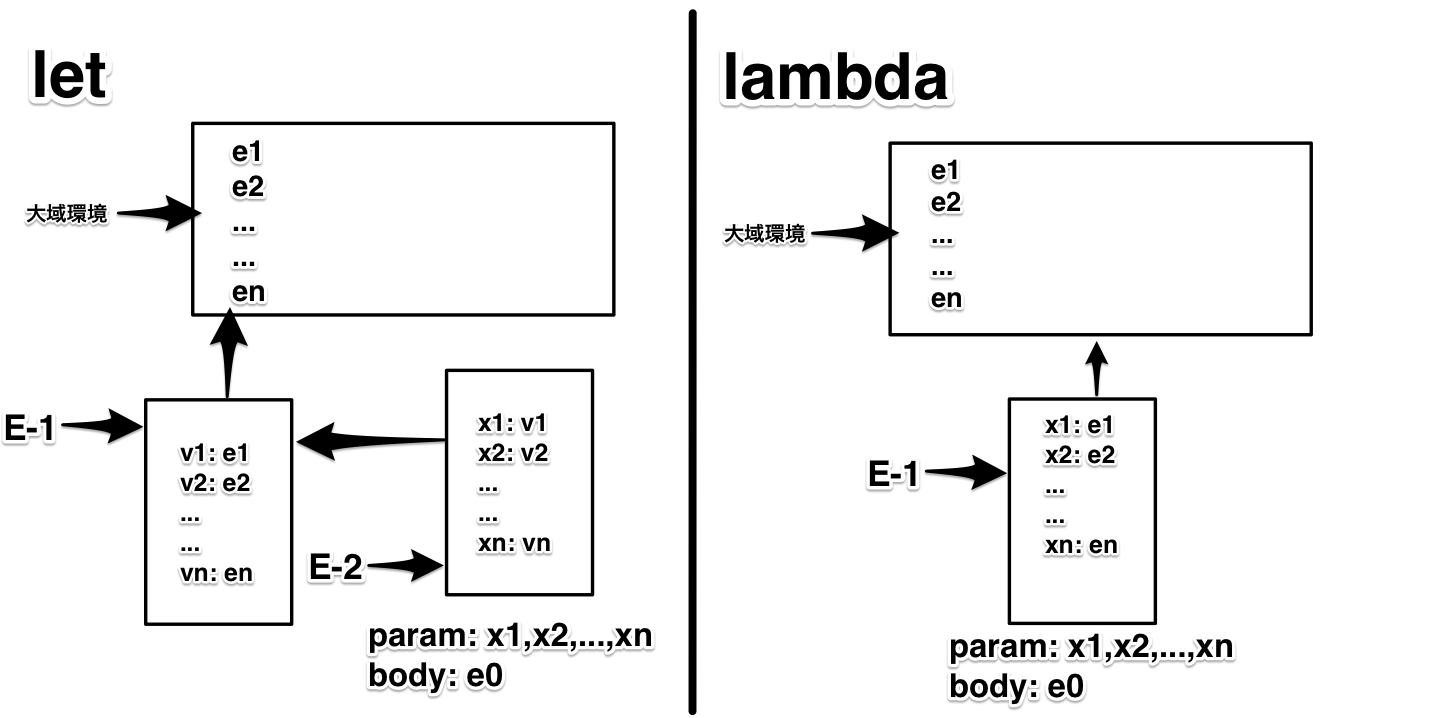
\includegraphics[width=15cm]{let-lambda.eps}
\end{document}

